\documentclass{article}

\usepackage[main]{neurips_2026}
% \usepackage[final,main]{neurips_2026}

\usepackage[utf8]{inputenc}
\usepackage{natbib}
\usepackage[T1]{fontenc}
\usepackage{hyperref}
\usepackage{url}
\usepackage{booktabs}
\usepackage{amsfonts}
\usepackage{amsmath}
\usepackage{nicefrac}
\usepackage{xcolor}
\usepackage{graphicx}
\usepackage{multirow}
\usepackage{subcaption}
\graphicspath{{figures/}}

% Review markup (blueline pass). \chg = blue (earlier pass);
% \rev = green (this revision pass); \cmt = green italic reviewer comment.
\newcommand{\chg}[1]{\textcolor{blue!70!black}{#1}}
\newcommand{\rev}[1]{\textcolor{green!45!black}{#1}}
\newcommand{\cmt}[1]{\textcolor{green!45!black}{\textit{[Reviewer comment: #1]}}}

\title{GORGO: Online Tuning for Cross-Region Network-Aware LLM Serving}

\author{Anonymous Author(s)}

\begin{document}

\maketitle

\begin{abstract}
Increasingly, LLM inference services proxy client requests to engine replicas distributed globally.
Load-balancing policies must jointly account for
factors including KV-cache locality, replica load, and variable network latency when
optimizing for metrics like latency and TTFT.
However, existing systems only evaluate a subset of these factors in their cost
model, leading to uneven concentrations of load and KV-cache across replicas. We
present GORGO, a proxy architecture that holistically factors network latency,
prefill cost, and queueing delay using tunable parameters. Since open-source chat
datasets such as LMSYS-Chat-1M and WildChat-4.8M lack long-context, high
prefix-reuse data, we release a synthetic dataset, ARTChat-411k, from
long-context production metadata. On a tuning window from ARTChat-411k,
evolutionary strategies guide the GORGO policy's parameters to directly optimize
p95 TTFT. During held-out evaluation windows, we fix the parameter values learned
from tuning and improve p95 TTFT by 8--15\% and end-to-end (E2E) latency by
15--31\% over baseline load balancing policies simple session affinity and prefix-cache.
Code can be found at \href{https://github.com/Arcadia-Research-Team/GORGO}{https://github.com/Arcadia-Research-Team/GORGO}.
\end{abstract}

% -----------------------------------------------------------------------
\section{Introduction}
\label{sec:intro}
% -----------------------------------------------------------------------

In LLM serving systems, perceived latency to the user is dominated by the time-to-first-token (TTFT). On a single replica, TTFT is dominated by three costs: prefill time, round trip time (RTT) from client (proxy) to replica, and queueing delay behind in-flight requests. Prefix-caching, which is enabled in modern inference engines SGLang \citep{sglang2024} and vLLM \citep{vllm2023}, eliminates the prefill cost of previous turns in a multi-turn conversation. As LLM context windows increase in length, the time saved by prefix caching 90\% of a prompt with 100,000 tokens reduces the prefill cost to 10,000 tokens and decreases TTFT substantially.

Since modern LLM deployments proxy requests to inference engines across regions, the cost savings of prefix-caching depend on choosing a replica with the request session's prefix. Popular routing policies such as consistent hashing and prefix reuse aim to distribute load evenly while creating affinity between a session's requests and replica(s) to maximize KV-cache reuse \citep{karger1997consistent, chord2003, sglang2024, skywalker}. In compute-constrained regimes, bursty workloads can saturate a high-affinity replica, causing head-of-line (HOL) queueing delays from decode memory contention and negating cost savings from prefix-cache reuse. Routing policies that holistically evaluate all costs related to TTFT can maintain high prefix-cache reuse while minimizing the negative effects of load saturation and heterogeneous network latency.

Existing load balancing policies such as least-load, session affinity, and prefix-reuse may account for replica load or KV-cache hit rate; however, no existing policies consider network latency in cross-region scenarios, which can range on the order of 10ms to 1s (Figure~\ref{fig:rtt}). GORGO's routing policy accounts for all three TTFT costs, normalizes the units of measurement via tunable parameters, and jointly optimizes parameters through online tuning on real user workloads. To tune and stress-test different routing policies, in (\S\ref{sec:characterization}) we compile a LLM traffic trace from real production requests with high prefix-reuse and long-context prompts. The trace follows Mooncake's FAST'25 format \citep{qin2024mooncake} containing per-request timestamps, which can be linearly scaled to simulate variable saturation profiles.

We benchmark GORGO on a series of user workloads from ARTChat-411k, our sensitized production Mooncake trace, and sweep across variable time scales to effectively saturate replicas without simulating unrealistic HOL queueing delay. Over existing load balancing policy baselines, GORGO jointly balances optimal TTFT with request concentration across replicas. Under the continuous batching paradigm, the ES-driven hillclimb tuner exploits warmer replicas close to the proxy and dramatically reduces TTFT at the cost of end-to-end (E2E) latency. We map the pareto frontier of request concentration across replicas, which explodes E2E latency for unbalanced distributions, and TTFT. Our contributions help contextualize the performance of LLM proxy routing policies in real-world user workloads, and (\S\ref{sec:results}) lists a case-by-case scenario of when one would want to use aforementioned baseline policies, the online GORGO policy, and offline GORGO with held-out weights. Finally, we show how conditioning the GORGO cost model on proxy-recorded replica load mitigates subversion of TTFT via continuous batching and slashes request latency across a panoply of metrics.

% -----------------------------------------------------------------------
\section{GORGO}
\label{sec:method}
% -----------------------------------------------------------------------

\subsection{Cost Model}

TTFT \rev{can be decomposed into} three different costs: network latency, prefill time, and queueing delay \citep{banaserve2025}. The KV-Cache, which stores key-value pairs of input sequences, removes redundant prefill computation for user sequences sharing a prefix with previously computed sequences \citep{sglang2024}. In a cross-region deployment setting, for an inference engine replica $i$ holding a set of cached token prefixes $c_i$, the cost of TTFT can be defined as the following function, where $x_r$ is the input sequence of tokens for a request $r$ and the prefill time depends only on the set difference $(x_r \setminus c_i)$, the tokens in $x_r$ not already cached on $i$:

\begin{equation}
\mathrm{TTFT} = T_{\texttt{network}}(i) + T_{\texttt{queue}}(i) + T_{\texttt{prefill}}(x_r \setminus c_i)
\label{eq:ttft}
\end{equation}

Theoretically, $T_{\texttt{network}}$ and $T_{\texttt{queue}}$ correspond with round trip time from a client to server and the duration of request processing ahead of the incoming request $r$. However, modern inference engines support batching requests continuously in order to minimize waiting for completion of previous request processing \citep{orca}. While continuous batching allows admission of a new request into the currently running batch, the batch size is still bounded by a maximum number of concurrent requests and the available KV-cache budget, a critical knob that governs how much load a replica can admit before further requests wait in a queue \citep{vllm2023}.

In a distributed system, the temporal delay of retrieving queueing metrics from an engine replica makes cost evaluation challenging. We represent the input to $T_{\texttt{queue}}$ as the total number of tokens of requests without a completion event on the client proxy. $T_{\texttt{network}}$ is measured trivially as the exponential weighted moving average of a ping's round trip time from client proxy to server.
\begin{equation}
\mathrm{TTFT} = T_{\texttt{network}}(\mathrm{RTT}_i) + T_{\texttt{queue}}\left(i, \sum_{j=1}^{n_r} x_j\right) + T_{\texttt{prefill}}(x_r \setminus c_i)
\end{equation}

\bigskip
\subsection{GORGO Proxy Design}

The GORGO proxy routes client requests to the engine replica with the minimum calculated cost from \rev{Equation~\ref{eq:score}}, parameterized by weights $W_{\texttt{rtt}}$, $W_{\texttt{prefill}}$, and $W_{\texttt{queue}}$. These parameters weight the inputs $T_{\texttt{network}}$, $T_{\texttt{queue}}$, and $T_{\texttt{prefill}}$, which unfairly mixes the units of time and tokens, to normalize the correlated costs of latency, prefill cost, and queueing time on TTFT. The weight of $T_{\texttt{prefill}}$ is fixed to 1 because GORGO proxy makes routing decisions based on relative replica cost: only the ratio of weights matters in this design.
\begin{equation}
\mathrm{TTFT} = W_{\texttt{rtt}} * T_{\texttt{network}}(\mathrm{RTT}_i) + W_{\texttt{queue}} * T_{\texttt{queue}}\left(i, \sum_{j=1}^{n_r} x_j\right) + T_{\texttt{prefill}}(x_r \setminus c_i)
\label{eq:score}
\end{equation}

GORGO proxy uses a simple (1+1) evolutionary strategy to tune weights $W_{\texttt{rtt}}$ and $W_{\texttt{queue}}$ on the objective function, P95 TTFT.
Each parent weight $x_{t,k}$ is perturbed multiplicatively in log-space by a normal random variable $z_k$ times step size $\sigma$, and the new offspring weight $x_k'$ is clamped to values in the hyperparameter range $[lo_k, hi_k]$ where $lo_k > 0$ and $hi_k > 0$.

\begin{equation}
x_k' = \mathrm{clip}\left(\exp(\ln(x_{t,k}) + \sigma_t * z_k), [lo_k, hi_k]\right)
\end{equation}

When $x'$ beats the parent weight $x_t$ on the objective metric, the incumbent weight $x_{t+1}$ is updated to $x'$, and $\sigma$ is adjusted to maintain Rechenburg's 1/5 success rate of 1 accepted offspring for every 5 offspring.

% -----------------------------------------------------------------------
\section{Workload Characterization}
\label{sec:characterization}
% -----------------------------------------------------------------------

Routing policies that perform well on short, low-reuse prompts may perform
differently on long, high-reuse prompts because the prefill term in TTFT scales
with uncached input tokens. We measure three datasets along the same axes:
request length, conversational structure, and token-weighted prefix reuse.

\paragraph{Datasets.}
\textbf{LMSYS-Chat-1M} \citep{lmsys2024} is a dataset of one million chatbot conversations from a publicly hosted demo of a Vicuna model and the ChatbotArena website. \textbf{WildChat-4.8M} \citep{wildchat2024} is a corpus
of 3.2M ChatGPT-proxy conversations grouped by client IP. Our \textbf{ARTChat-411k
trace} contains chat completion requests from a production
GLM 5.1 model endpoint hosted by an industry company\citep{glm2024}. It contains 411{,}169 requests across 4{,}984 distinct
users, yielding $\sim$82 requests per user on average. We used the request metadata for real-world timestamps and tokenized request bodies for reuse calculation.

We measure prefix reuse with a token-weighted prefix trie that ingests each
request's tokenized message sequence in arrival order, partitioned by user where
the dataset carries user identity. The trie reports \textit{intra-user savings}
(fraction of tokens matching a prefix from the same user's prior requests),
\textit{cross-user savings} (additional fraction from pooling across users), and
\textit{global savings} (sum). LMSYS does not carry user identity, so we report
only the global figure.

\begin{table}[t]
\centering
\small
\caption{Workload characterization. Token counts use the same byte-pair
  tokenizer in all rows. Reuse percentages are token-weighted prefix-trie
  savings as described in \S\ref{sec:characterization}.}
\label{tab:datasets}
\begin{tabular}{lrrrrr}
\toprule
Dataset & Total reqs & Users & Avg input tokens & Intra-user reuse & Global reuse \\
\midrule
LMSYS-Chat-1M & 1{,}000{,}000 & --- & 467 & --- & 9.0\% \\
WildChat-4.8M & 3{,}199{,}860 & 1{,}833{,}730 & 2{,}925 & 5.3\% & 34.4\% \\
ARTChat-411k & 411{,}169 & 4{,}984 & 21{,}043 & 53.7\% & 55.3\% \\
\bottomrule
\end{tabular}
\end{table}

Three contrasts stand out (Table~\ref{tab:datasets}, Figure~\ref{fig:dataset_combined}). \textit{Request length}:
ARTChat-411k prompts are 45$\times$ longer than LMSYS and 7$\times$ longer than
WildChat. At typical rates, prefill on a 21{,}000-token uncached prompt takes on the order of seconds. 

\textit{User concentration}: ARTChat-411k has 82 requests per user on
average; WildChat has 1.7; LMSYS does not carry user identifiers, so intra-user
statistics cannot be computed. Intra-user reuse depends
on returning users, which the public sets simply do not have. \textit{Reuse
magnitude}: 53.7\% of ARTChat-411k tokens are part of a prefix seen earlier from the
same user (5.3\% for WildChat, essentially zero for LMSYS). The bulk of
WildChat's 34.4\% global reuse comes from cross-user shared structure (chat
templates, viral prompts), not sustained per-user dialogue.
Thus, for routing, LMSYS and WildChat live in a regime where prefix-aware policies
have little to win. On ARTChat-411k, a strategy that lands a user on a replica that
has seen their conversation can save more than half of the prefill.

\begin{figure}[t]
\centering

\includegraphics[width=\linewidth]{dataset_combined.png}
\caption{\textit{Left}: Token composition per dataset. ARTChat-411k's reuse
  is overwhelmingly intra-user (54\%), reflecting multi-turn dialogue;
  WildChat's is predominantly cross-user (29\%, shared templates); LMSYS
  has minimal reuse (9\%, all cross-user). \textit{Right}: Radar chart
  with six axes normalized to the dataset maximum. ARTChat-411k dominates on
  every axis relevant to routing: long prompts, high multi-turn density,
  concentrated users, and strong intra-user prefix reuse.}
\label{fig:dataset_combined}
\end{figure}

\paragraph{Experimental windows.}
We tune on a high-diversity 30-minute window from ARTChat-411k traffic on April
5th, 2026: 16:15--16:45 UTC (W1). We then freeze the learned parameters and
evaluate on two non-consecutive, held-out windows drawn from later days and
time-of-day regimes: April 6th, 15:05--15:35 UTC (W2a), and April 7th,
19:45--20:15 UTC (W2b). This split tests whether parameters learned from one
high-diversity window generalize to later traffic rather than simply carrying
over to an adjacent interval. The two evaluation windows were selected from the
7-day trace for high user diversity and multi-turn density while avoiding
single-user-dominated bursts. Traces are replayed at original arrival speed and
pre-filtered to 24{,}000 input tokens. Output is capped at 128 tokens to
prevent decode from dominating latency.

% -----------------------------------------------------------------------
\section{Experimental Setup}
\label{sec:setup}
% -----------------------------------------------------------------------

\paragraph{Hardware and software.}
Each policy runs on its own dedicated three-replica fleet so routing decisions
cannot warm or cool another policy's caches. Each fleet consists of one 2$\times$L40S
SGLang \citep{sglang2024} server (tensor-parallel 2, 96\,GB VRAM per replica)
in each of Asia (Seoul), Europe (Frankfurt), and US East (Ashburn), serving
Qwen3.5-35B-A3B-FP8 \citep{qwen3technical}. The model's native context window
is 32{,}768 tokens; we cap workload input at 24{,}000 tokens to leave KV headroom
for in-flight batches. A CPU proxy in US East (Ashburn) hosts the routing policy and
replays the trace.

\paragraph{Cross-region RTT distribution.}
Probed from the US East proxy over the Apr~5 16:15--16:45 tuning window,
EWMA-smoothed RTT to the US East (Ashburn) replica is 30--45\,ms
(mean $37\pm8$\,ms), to Frankfurt 200--390\,ms (mean $279\pm80$\,ms), and to
Seoul 260--700\,ms (mean $456\pm138$\,ms). The wide Seoul swing reflects
routing-table churn along the trans-Pacific path during the trace, while
Ashburn stays near-constant. Mean RTT spans a 12$\times$ range across regions,
widening to $\sim$23$\times$ at the Seoul peak.
Figure~\ref{fig:rtt} shows the full RTT time series over the tuning window.

\begin{figure}[t]
\centering
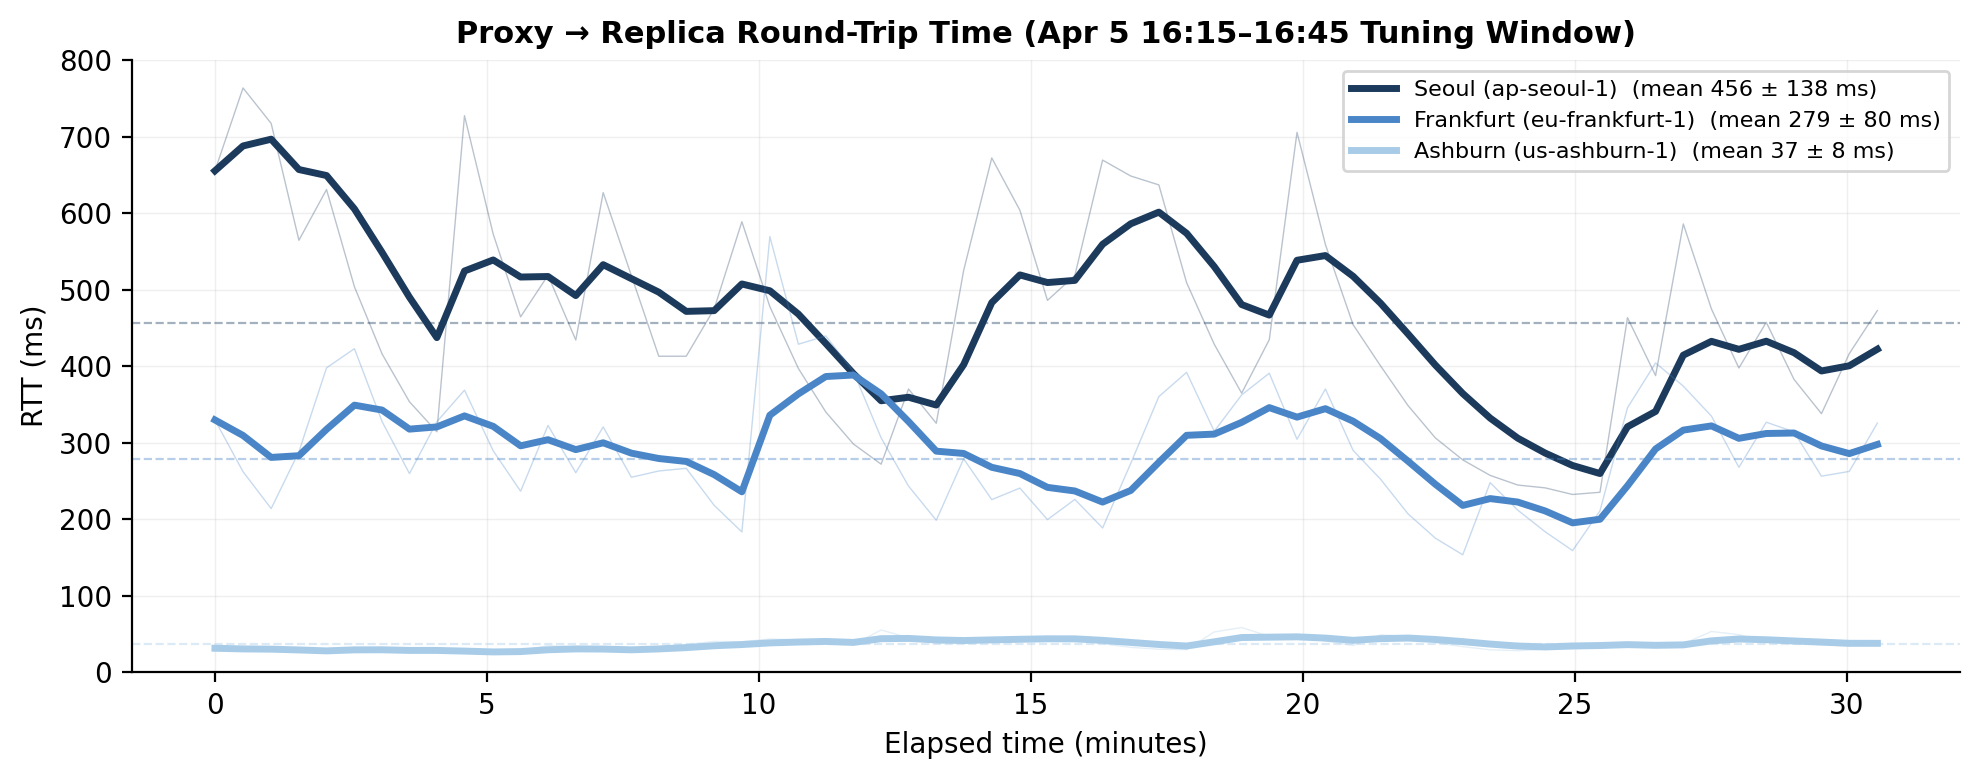
\includegraphics[width=\linewidth]{rtt_timeseries_apr5_1615_1645.png}
\caption{Proxy-to-replica RTT over the Apr~5 16:15--16:45 tuning window. Bold
  lines show the EWMA-smoothed signal ($\alpha{=}0.3$) that GORGO uses for
  routing; faint lines show raw probe samples. Dashed lines show per-replica
  means (Seoul 456\,ms, Frankfurt 279\,ms, Ashburn 37\,ms). Seoul swings widely
  from trans-Pacific routing-table churn; Frankfurt is moderately variable;
  Ashburn is near-constant. The wide cross-region spread motivates
  network-aware routing.}
\label{fig:rtt}
\end{figure}

\paragraph{Baselines, policies, and windows.}
We compare the three GORGO variants of \S\ref{sec:method}
(\texttt{gorgo-static}, \texttt{gorgo-autotune}, \texttt{gorgo-hillclimb})
against five baseline policies. \texttt{random} samples a replica uniformly per
request and serves as the lower bound. \texttt{least-request} routes to the
replica with the fewest in-flight requests, taking the larger of the proxy's
in-flight view and SGLang's scraped running-request count to bridge the
$\sim$10\,s staleness between metrics scrapes. \texttt{least-load} routes to the
replica with the lowest aggregate token-weighted load, summing running and
queued requests with used and queued KV tokens; it is heavier-signal than
least-request but cache-blind. \texttt{prefix-cache} is the longest-prefix-match policy of Preble
\citep{preble} as packaged in AIBrix \citep{aibrix2024}: it picks the replica
with the longest cached prefix match and falls back to least-request when the
running-request imbalance exceeds a soft threshold. \texttt{simple-session-affinity}
hashes the first 256 token IDs of the prompt modulo the number of replicas,
maximizing intra-user reuse but providing no load-escape mechanism. We evaluate
these six policies in each of two windows; all six fleets start
simultaneously at the same wall-clock time with the same input trace. W1 supplies
\texttt{gorgo-hillclimb} with uniform starting weights
($\mathrm{rtt\_weight}{=}1.0$, $\mathrm{prefill\_weight}{=}1.0$,
$\mathrm{load\_weight}{=}1.0$); W2 uses the weights that
\texttt{gorgo-hillclimb} learned during W1
($\mathrm{rtt\_weight}{\approx}0.39$, $\mathrm{prefill\_weight}{\approx}1.88$,
$\mathrm{load\_weight}{\approx}6.38$). \texttt{gorgo-static} in W2 deploys those
weights without further adjustment. Concurrency is 64 in-flight requests per proxy.

\paragraph{Metrics.}
For each policy and window we report TTFT p50, p95, and p99 over all successful
streaming responses. Traces are pre-filtered to the model's effective context
boundary; all policies achieve 100\% success rate in all windows.

% -----------------------------------------------------------------------
\section{Results}

\label{sec:results}
% -----------------------------------------------------------------------

\subsection{p95 TTFT Objective}
\label{sec:results:p95}

\paragraph{Results across three windows.}

\begin{table}[t]
\centering
\small
\caption{Decoded-trace results across three 30-minute windows. GORGO uses the
  2D cost model with weights $w_{\mathrm{rtt}}{=}0.276$, $w_{\mathrm{queue}}{=}0.5$,
  learned by $(1{+}1)$-ES on the Apr~5 tuning window and \emph{frozen} for both
  held-out windows. TTFT in ms, E2E p95 in s; bold is best in column within each
  window. The held-out windows are replayed within capacity for every policy
  (scheduling-slip p95 $\le 10$\,ms).}
\label{tab:results}
\begin{tabular}{lrrrr}
\toprule
Policy & TTFT p50 & TTFT p95 & TTFT p99 & E2E p95 \\
       & (ms)     & (ms)     & (ms)     & (s)     \\
\midrule
\multicolumn{5}{l}{\textit{Tuning window --- Apr~5 16:15--16:45 (in-sample, full load; $n{=}7{,}195$)}} \\
\midrule
\textbf{GORGO }     & \textbf{673}    & 2{,}514          & \textbf{4{,}473} & \textbf{8.91}  \\
simple-session-affinity & 712             & \textbf{2{,}428} & 5{,}190          & 18.27 \\
least-load              & 763             & 2{,}447          & 4{,}349          & 13.69 \\
least-request           & 968             & 3{,}970          & 7{,}012          & 16.62 \\
prefix-cache            & 1{,}477         & 6{,}784          & 9{,}613          & 22.63 \\
\midrule
\multicolumn{5}{l}{\textit{Held-out eval --- Apr~6 15:05--15:35, half load ($n{=}7{,}630$)}} \\
\midrule
\textbf{GORGO }     & \textbf{491}    & \textbf{1{,}584} & \textbf{2{,}222} & \textbf{3.29} \\
simple-session-affinity & 627             & 1{,}875          & 3{,}056          & 4.75 \\
least-load              & 616             & 1{,}818          & 2{,}885          & 4.06 \\
least-request           & 634             & 1{,}852          & 2{,}484          & 3.99 \\
prefix-cache            & 574             & 1{,}798          & 2{,}750          & 4.95 \\
\midrule
\multicolumn{5}{l}{\textit{Held-out eval --- Apr~7 19:45--20:15, third load ($n{=}8{,}663$)}} \\
\midrule
\textbf{GORGO }     & \textbf{386}    & \textbf{1{,}377} & \textbf{1{,}973} & \textbf{3.34} \\
simple-session-affinity & 439             & 1{,}495          & 2{,}313          & 3.90 \\
least-load              & 480             & 1{,}637          & 2{,}294          & 4.04 \\
least-request           & 509             & 1{,}724          & 2{,}485          & 4.40 \\
prefix-cache            & 516             & 1{,}830          & 2{,}801          & 11.98 \\
\bottomrule
\end{tabular}
\end{table}

Table~\ref{tab:results} reports all three decoded-trace windows under the frozen
2D weights ($w_{\mathrm{rtt}}{=}0.276$, $w_{\mathrm{queue}}{=}0.5$). On the
in-sample Apr~5 tuning window---at full arrival rate, where every policy is
saturated---GORGO wins TTFT p50 and p99 and cuts E2E p95 by 34.9\% over the best
baseline (8.91\,s vs.\ 13.69\,s), trailing \texttt{simple-session-affinity} by
only 3.5\% on TTFT p95. On both held-out windows---Apr~6 at half load and Apr~7
at third load, each within capacity for all five policies---GORGO
\emph{sweeps every metric}: on Apr~6, TTFT p95 is 15.5\% better than
\texttt{simple-session-affinity} (1{,}584 vs.\ 1{,}875\,ms) and E2E p95 is
30.8\% better (3.29 vs.\ 4.75\,s); on Apr~7, TTFT p95 is 7.9\% better
(1{,}377 vs.\ 1{,}495\,ms) and E2E p95 is 14.5\% better (3.34 vs.\ 3.90\,s).
The weights, learned once on Apr~5, transfer to later days and times of day
without re-tuning. Figure~\ref{fig:ttft_multibar} visualizes the TTFT p95
comparison across the three windows, and Figure~\ref{fig:es_convergence} shows
the tuning run that produced the weights.

\begin{figure}[t]
\centering

\includegraphics[width=\linewidth]{ttft_multibar.png}
\caption{\rev{TTFT p95 across the three load-sweep windows
  (Table~\ref{tab:results}), GORGO (gold) vs.\ baselines under the frozen 2D
  weights. At full load (Apr~5, saturated) GORGO is within 3.5\% of the best
  baseline; as load backs off to half (Apr~6) and a third (Apr~7) of capacity,
  GORGO becomes the lowest-p95 policy in every window, the advantage widening as
  the fleet gains slack.}}
\label{fig:ttft_multibar}
\end{figure}

\begin{figure}[t]
\centering
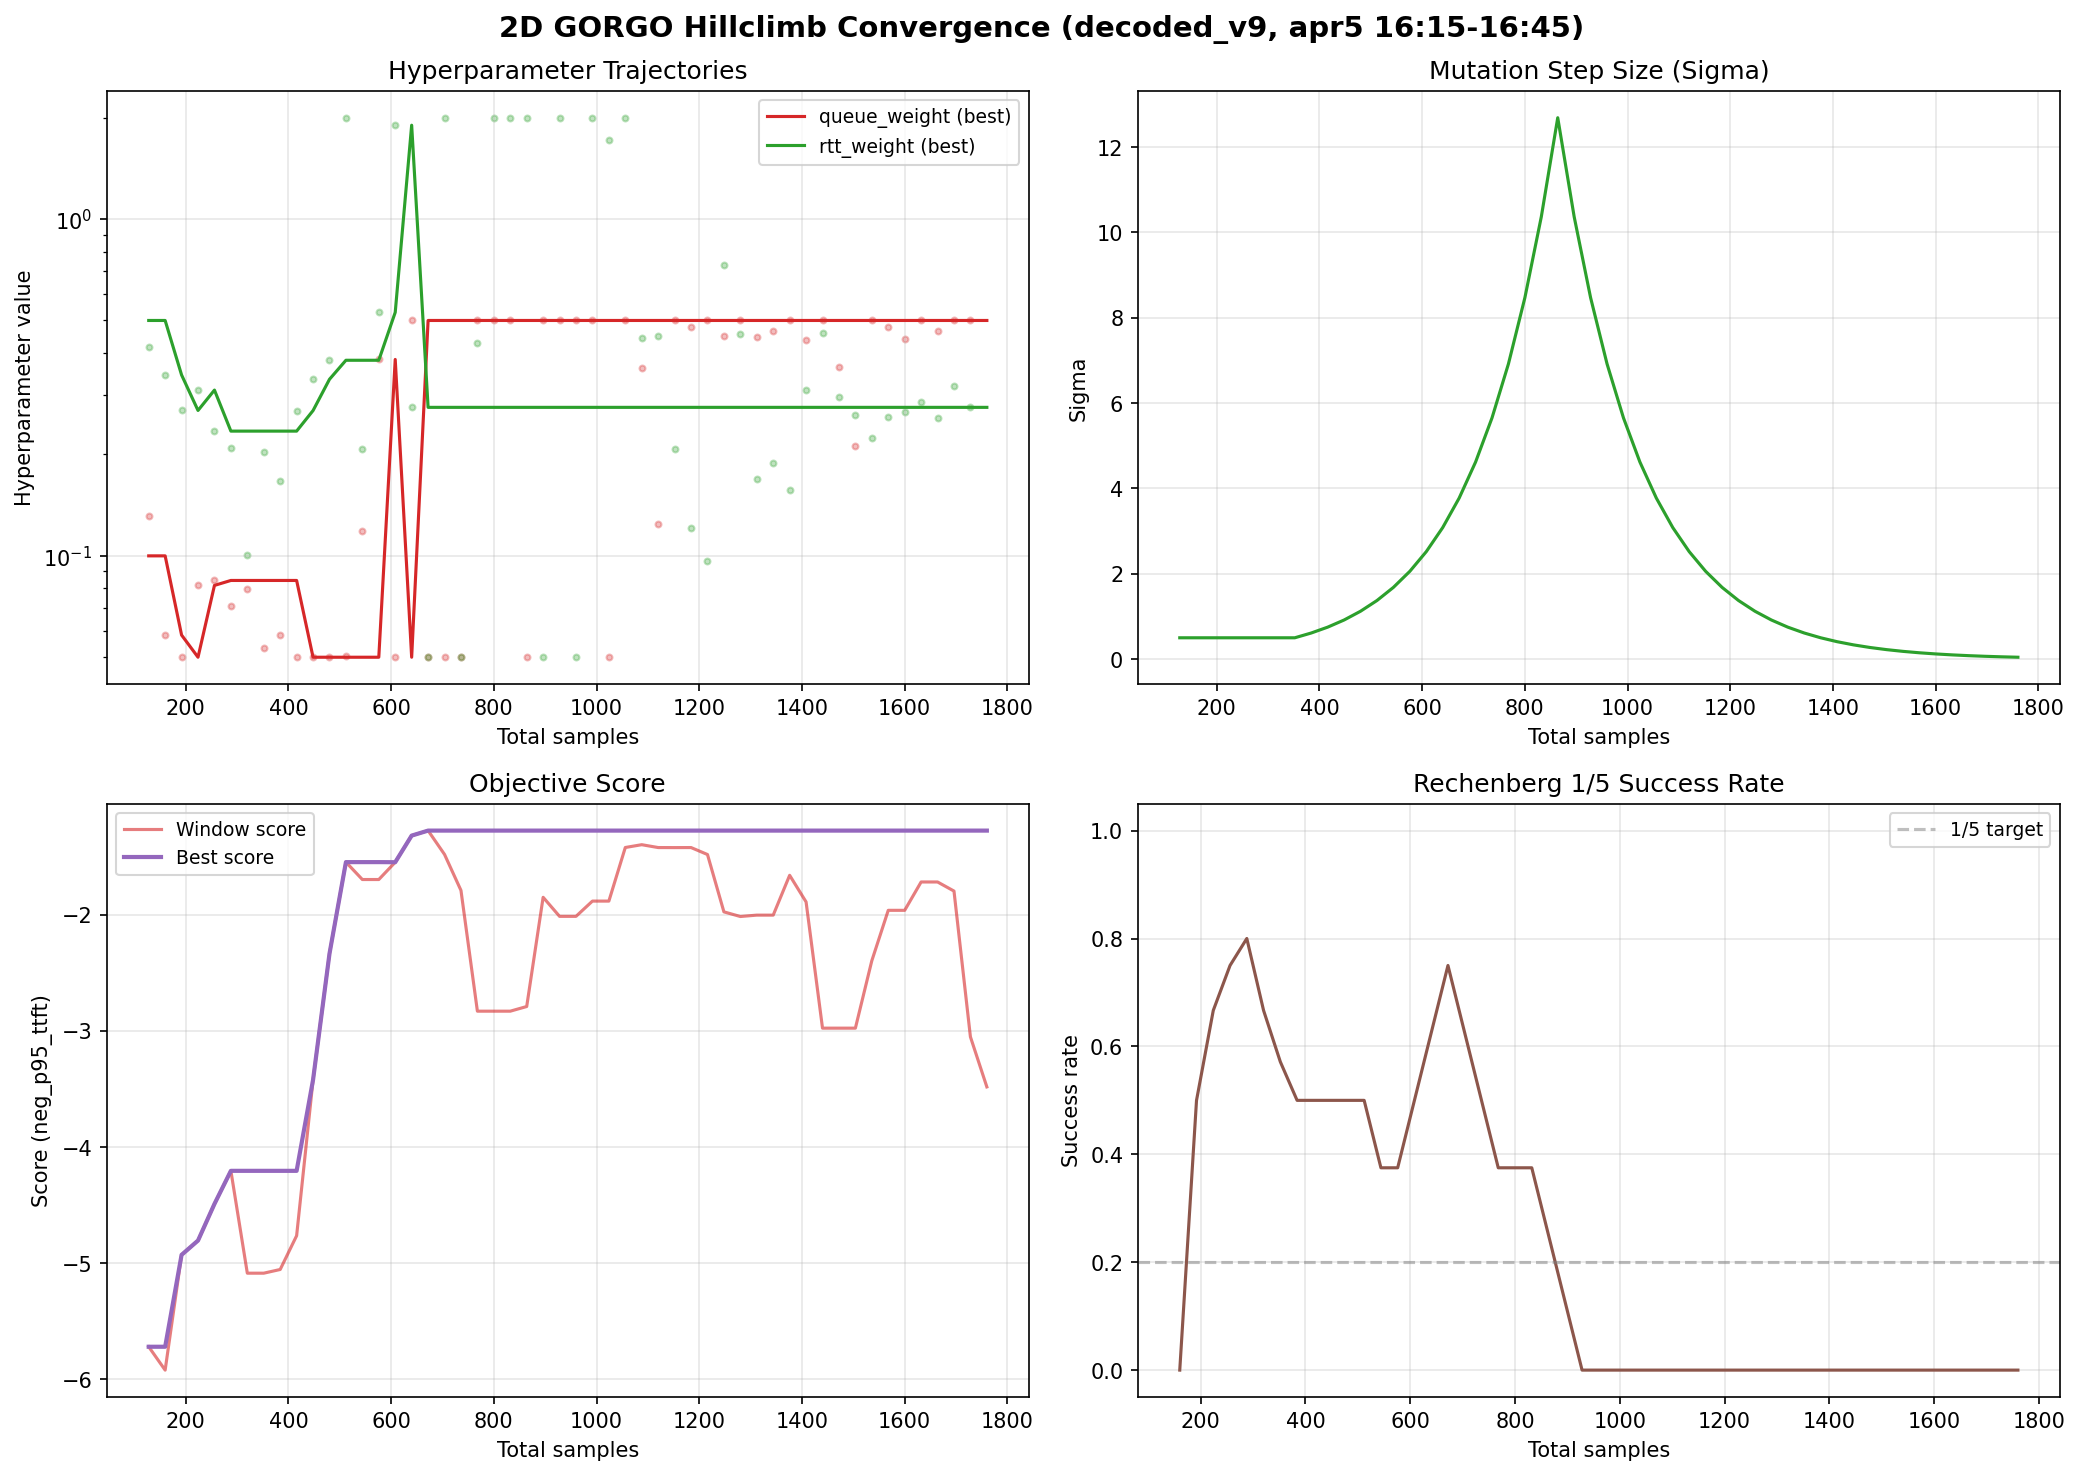
\includegraphics[width=\linewidth]{tune_convergence_2d_v9.png}
\caption{$(1{+}1)$-ES convergence on the Apr~5 tuning window (p95 TTFT objective).
  \textit{Top-left}: best-incumbent weight trajectories---$w_{\mathrm{queue}}$
  rails at its 0.5 ceiling (maximal load avoidance) while $w_{\mathrm{rtt}}$
  settles near 0.28; dots show ES proposals. \textit{Top-right}: step size
  $\sigma$ rises then decays as the search converges. \textit{Bottom-left}:
  objective (negative p95 TTFT) climbs from $-5.9$ to $-1.2$.
  \textit{Bottom-right}: acceptance rate falls toward the 1/5 target.}
\label{fig:es_convergence}
\end{figure}

% -----------------------------------------------------------------------
\subsection{p50 TTFT Objective}
\label{sec:results:p50}

\cmt{This p50 subsection and the Objective-Sensitivity table
(Table~\ref{tab:weights_compare}) still report the OLD 3-weight model on the apr2
windows ($w_{\mathrm{rtt}}/w_{\mathrm{prefill}}/w_{\mathrm{load}}=0.39/1.88/6.38$),
which is inconsistent with the 2D results above (2 free weights
$w_{\mathrm{rtt}},w_{\mathrm{queue}}$ on decoded Apr~5--7). To reconcile: re-run
the p50 objective under the 2D model, or relocate this to an appendix as the
3-weight precursor. The real-trace numbers here are Modal-only (not locally
verifiable).}

To test whether the learned weights depend on the objective percentile, we
re-run W1 tuning with a p50 TTFT objective (same trace, same hyperparameter
ranges).

\begin{table}[t]
\centering
\small
\caption{ARTChat-411k W1 with p50 TTFT objective (tuning window, 00:30--01:00 UTC,
  April 2nd 2026). Same trace and ranges as the p95 run.
  $n{=}2{,}095$ requests per policy; 100\% success rate.}
\label{tab:w1_p50}
\begin{tabular}{lrrr|rrr|r}
\toprule
 & \multicolumn{3}{c|}{TTFT (s)} & \multicolumn{3}{c|}{E2E (s)} & Succ. \\
Policy & p50 & p95 & p99 & p50 & p95 & p99 & \% \\
\midrule
\textbf{gorgo-hillclimb} & \textbf{0.163} & \textbf{0.943} & 2.185 & 1.45 & 2.40 & 3.95 & 100 \\
simple-session-affinity   & 0.196          & 0.988          & \textbf{1.654} & 1.48 & 2.61 & 3.47 & 100 \\
least-request             & 0.207          & 1.102          & 1.934 & \textbf{1.24} & \textbf{2.10} & \textbf{3.07} & 100 \\
least-load                & 0.264          & 1.079          & 1.874 & 1.40 & 2.38 & 2.92 & 100 \\
random                    & 0.274          & 1.186          & 2.021 & 1.27 & 2.33 & 3.24 & 100 \\
prefix-cache              & 0.287          & 1.052          & 1.773 & 1.31 & 2.34 & 3.32 & 100 \\
\bottomrule
\end{tabular}
\end{table}

The p50-tuned ES converged to $w_{\mathrm{rtt}}{=}1.21$,
$w_{\mathrm{prefill}}{=}0.52$, $w_{\mathrm{load}}{=}1.69$---a qualitatively
different operating point from the p95 run. \texttt{gorgo-hillclimb} achieves
0.163\,s p50 TTFT (16.8\% gap over \texttt{simple-session-affinity}) and
0.943\,s p95 TTFT (4.5\% gap). However, the RTT-first routing concentrates
traffic on the nearest replica, degrading E2E: p95 E2E is 2.40\,s, 14.1\%
worse than \texttt{least-request} (2.10\,s). This tradeoff---better median TTFT
at the cost of E2E---is the mirror image of the p95 policy, which wins both.

\begin{figure}[t]
\centering
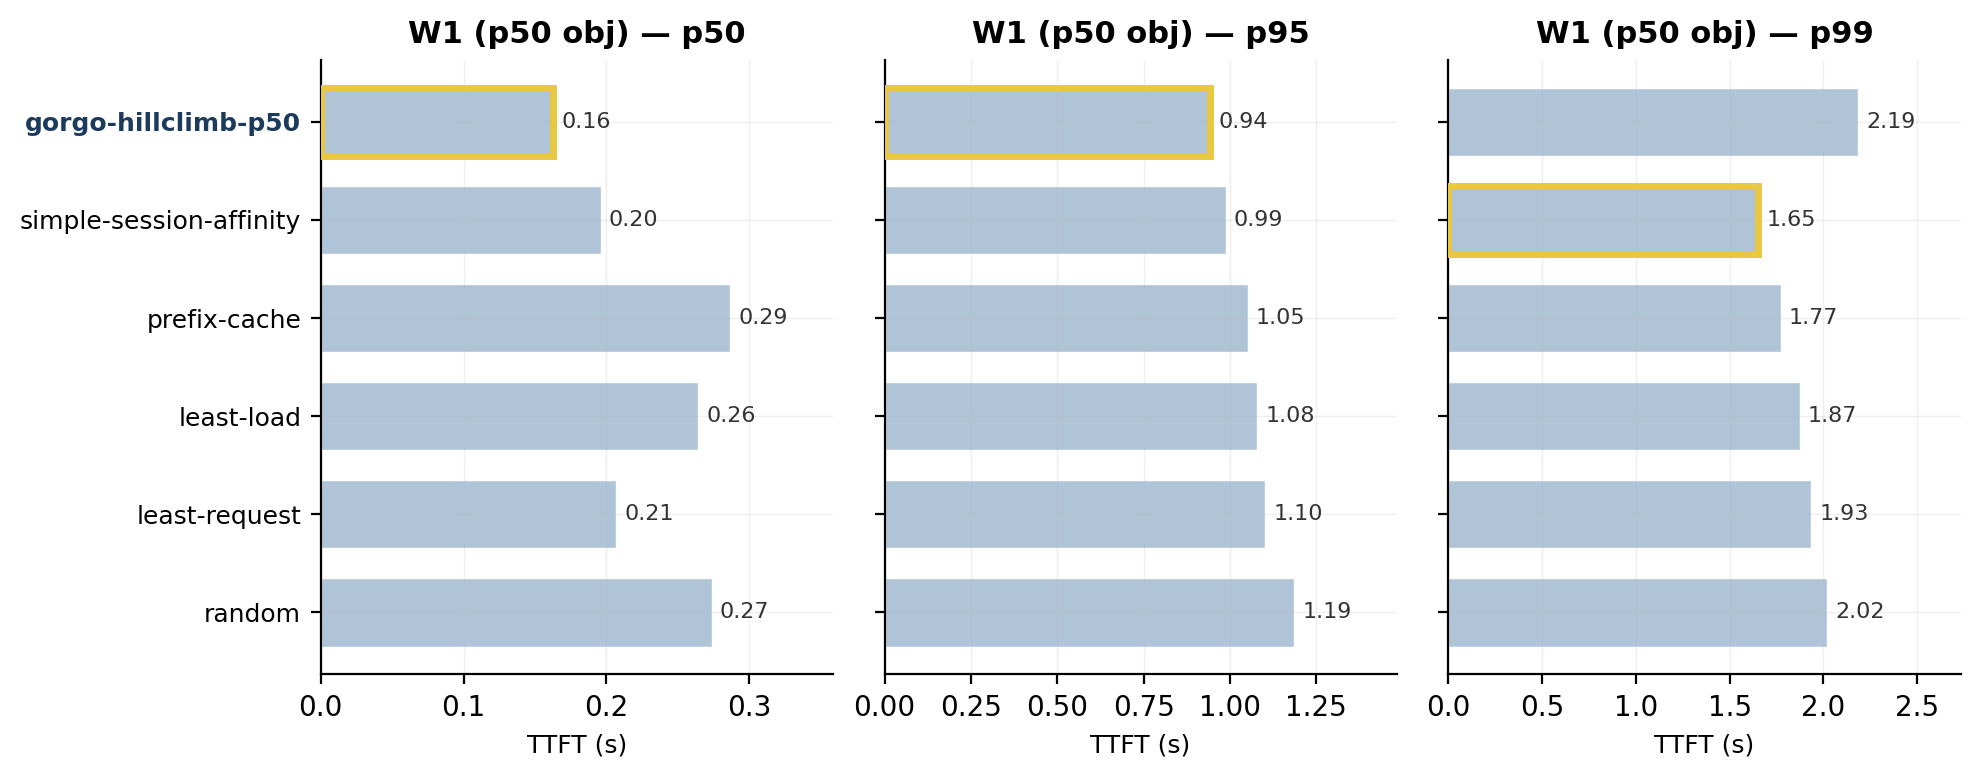
\includegraphics[width=\linewidth]{ttft_bars_p50_w1.png}
\caption{W1 TTFT with p50 objective. \texttt{gorgo-hillclimb} (gold outline)
  achieves the best p50 (0.163\,s) by prioritizing RTT over cache.}
\label{fig:ttft_bars_p50}
\end{figure}

\paragraph{Held-out evaluation.}

\begin{table}[t]
\centering
\small
\caption{p50-objective W2a (held-out nighttime, 01:00--01:30 UTC, April 2nd 2026).
  \texttt{gorgo-static} deploys the p50-tuned weights ($w_{\mathrm{rtt}}{=}1.21$,
  $w_{\mathrm{prefill}}{=}0.52$, $w_{\mathrm{load}}{=}1.69$).
  $n{=}2{,}207$ requests per policy; 100\% success rate.}
\label{tab:w2_p50}
\begin{tabular}{lrrr|rrr|r}
\toprule
 & \multicolumn{3}{c|}{TTFT (s)} & \multicolumn{3}{c|}{E2E (s)} & Succ. \\
Policy & p50 & p95 & p99 & p50 & p95 & p99 & \% \\
\midrule
\textbf{gorgo-static}    & \textbf{0.157} & \textbf{0.961} & \textbf{1.776} & 1.42 & 2.42          & 3.27          & 100 \\
simple-session-affinity   & 0.206          & 0.995          & 1.960          & 1.56 & 2.67          & 3.45          & 100 \\
least-request             & 0.238          & 1.180          & 1.812          & \textbf{1.25} & \textbf{2.27} & \textbf{3.27} & 100 \\
least-load                & 0.289          & 1.298          & 2.052          & 1.41 & 2.57          & 3.27          & 100 \\
prefix-cache              & 0.290          & 1.160          & 1.944          & 1.51 & 2.51          & 8.65          & 100 \\
\bottomrule
\end{tabular}
\end{table}

In W2a, \texttt{gorgo-static} with p50-tuned weights sweeps TTFT: p50
(0.157\,s, 23.8\% gap over \texttt{simple-session-affinity}), p95 (0.961\,s,
3.4\% gap), and p99 (1.776\,s). E2E p95 is 2.42\,s---6.6\% worse than
\texttt{least-request} (2.27\,s), consistent with the RTT-first routing
tradeoff observed in W1.

\begin{table}[t]
\centering
\small
\caption{p50-objective W2b (held-out midday diurnal, 12:30--13:00 UTC, April 2nd 2026).
  $n{=}3{,}071$ requests per policy; 100\% success rate.}
\label{tab:w2b_p50}
\begin{tabular}{lrrr|rrr|r}
\toprule
 & \multicolumn{3}{c|}{TTFT (s)} & \multicolumn{3}{c|}{E2E (s)} & Succ. \\
Policy & p50 & p95 & p99 & p50 & p95 & p99 & \% \\
\midrule
\textbf{gorgo-static}    & \textbf{0.188} & \textbf{1.184} & \textbf{1.901} & 1.60 & 2.92          & 4.83          & 100 \\
simple-session-affinity   & 0.240          & 1.498          & 2.523          & 1.71 & 3.78          & 8.21          & 100 \\
random                    & 0.289          & 1.421          & 2.331          & \textbf{1.40} & 2.93          & 3.97          & 100 \\
prefix-cache              & 0.293          & 1.451          & 2.973          & 1.59 & 3.22          & 5.29          & 100 \\
least-request             & 0.293          & 1.345          & 2.167          & 1.36 & \textbf{2.68} & \textbf{3.83} & 100 \\
least-load                & 0.303          & 1.831          & 3.144          & 1.66 & 3.91          & 8.36          & 100 \\
\bottomrule
\end{tabular}
\end{table}

In W2b (midday), \texttt{gorgo-static} with p50-tuned weights wins TTFT p50
(0.188\,s, 21.7\% gap), p95 (1.184\,s, 12.0\% gap over \texttt{least-request}),
and p99 (1.901\,s, 12.3\% gap). E2E p95 is 2.92\,s, 8.9\% worse than
\texttt{least-request} (2.68\,s). The p50-tuned policy achieves stronger TTFT
p50 margins than the p95-tuned policy (21.7\% vs.\ 16.4\%) but pays a
consistent E2E penalty---the lower $w_{\mathrm{load}}{=}1.69$ (vs.\ 6.38)
provides less load balancing under the heavier midday traffic.

% -----------------------------------------------------------------------
\subsection{Objective Sensitivity: Weight Comparison}
\label{sec:results:objective}

Table~\ref{tab:weights_compare} compares the learned weights across objectives.

\begin{table}[t]
\centering
\small
\caption{Learned weights under different objective metrics, same tuning trace and
  hyperparameter ranges. The ES discovers qualitatively different operating
  points depending on which percentile it optimizes.}
\label{tab:weights_compare}
\begin{tabular}{lrrr}
\toprule
Objective & $w_{\mathrm{rtt}}$ & $w_{\mathrm{prefill}}$ & $w_{\mathrm{load}}$ \\
\midrule
neg\_p95\_ttft & 0.39 & 1.88 & 6.38 \\
neg\_p50\_ttft & 1.21 & 0.52 & 1.69 \\
\bottomrule
\end{tabular}
\end{table}

The p95 objective drives the policy toward cache-first routing
($w_{\mathrm{prefill}}{=}1.88$) with aggressive load avoidance
($w_{\mathrm{load}}{=}6.38$), because tail requests are the ones stuck behind
queues on cache-cold replicas. The p50 objective drives toward RTT-first
routing ($w_{\mathrm{rtt}}{=}1.21$, 3.1$\times$ larger), because the typical
request is short enough that network latency dominates over cache effects.
The p50-tuned policy achieves 0.163\,s p50 TTFT (vs.\ 0.180\,s for p95-tuned),
a 9\% improvement on the metric it optimizes.

% -----------------------------------------------------------------------


\section{Limitations}
\label{sec:limitations}
% -----------------------------------------------------------------------

\paragraph{p99 noise floor.}
Each window has $\approx\!2{,}100$--$2{,}200$ successful responses, so the p99
standard error is $\sigma_{\mathrm{TTFT}}/\sqrt{n\cdot 0.01\cdot 0.99}\approx
0.07$\,s. \cmt{Stale: the 1.626/1.702 values below match no table and refer to
the apr2 W2 window, which the p95 results no longer use (now the decoded
Apr~5--7 windows); reconcile or remove once p50/p99 are migrated to the 2D
results.} The W2 p99 gap between \texttt{gorgo-static} (1.626\,s) and
the next-best policy \texttt{prefix-cache} (1.702\,s) is 0.076\,s---just above
one SE---so the p99 win, while directionally consistent with p50 and p95, is not
individually significant at this sample size.

\paragraph{Scope of fleet.}
Each policy runs on its own dedicated three-replica fleet of identical GPUs. Multi-tenant sharing, heterogeneous hardware, and prefill/decode disaggregation \citep{distserve2024,splitwise2024} are not characterized here and would require additional cost terms. The score uses only HTTP-exposed metrics, not scheduler-internal signals \citep{kvflow2025,lpc2025} that could tighten the prefill estimate.

\paragraph{Live-tuning instability.}
Running the $(1{+}1)$-ES live can produce a heavy-tailed p99 excursion
because the negative-p95 objective does not penalize a single
bad-minute proposal fast enough. The freeze-for-production recommendation in
\S\ref{sec:results:p95} is therefore a safety property, not just a
convenience. Decode dynamics such as the effect of variable length decode and high memory consumption on load may impact live-tuning instability; exploring the impact of higher output token limits would be a direction for future work.

% -----------------------------------------------------------------------
\section{Related Work}
\label{sec:related}
% -----------------------------------------------------------------------

\paragraph{Prefix caches and reuse.}
RadixAttention in SGLang \citep{sglang2024} stores per-request KV state in a
radix tree; PagedAttention in vLLM \citep{vllm2023} enables prefix sharing
through paged memory. KVLink \citep{kvlink2025}, ChunkKV \citep{chunkkv2025},
KVFlow \citep{kvflow2025}, and Learned Prefix Caching \citep{lpc2025} improve
the single-replica cache but do not decide which replica serves a request.

\paragraph{Cross-replica routing and cross-region serving.}
Preble \citep{preble} introduces longest-prefix-match routing across replicas
with a load-balance fallback; AIBrix \citep{aibrix2024} packages a
production-grade variant of the same design and supplies the baseline we run.
Mooncake \citep{qin2024mooncake} is a KV-cache-centric architecture and the
source of our trace format. SkyServe \citep{skyserve} and SkyWalker
\citep{skywalker} address cross-region LLM serving at the placement and
spillover layers respectively, but treat per-request routing as out of scope.
k-LPM \citep{klpm2025} formulates LLM scheduling under TTFT constraints as
NP-hard. DLPM \citep{dlpm2025} targets fairness with locality. Llumnix
\citep{llumnix2024} migrates requests across replicas. Multi-LLM routers
\citep{routerwu2025} address model selection. \rev{CacheBlend
\citep{yao2024cacheblend} extends KV reuse beyond exact prefixes by selectively
recomputing cache for fused non-prefix chunks, but targets single-node reuse
rather than cross-replica routing.} DistServe \citep{distserve2024} and Splitwise
\citep{splitwise2024} disaggregate prefill from decode. GORGO is the first
single-router policy in this space that scores cache locality, replica load,
and wide-area latency in one cost and derives the cost weights from the
deployment's own per-request TTFT stream, with no engine modifications.

\paragraph{Online hyperparameter adaptation.}
Bayesian and bandit-based methods have been applied to serving configuration
\citep{routerwu2025}. For a 2-dimensional parameter space the $(1{+}1)$-ES
\citep{rechenberg1973} provides fast, overhead-free convergence with no
surrogate model.

% -----------------------------------------------------------------------
\section{Conclusion}
\label{sec:conclusion}
% -----------------------------------------------------------------------

Routing across LLM replicas is a three-signal decision balancing cache locality, replica
load, and wide-area latency, but production heuristics commit to one signal and
degrade when that stops being the limiting factor. We treat the three as
terms of an additive per-replica cost and let online TTFT feedback optimize 
scaling weights, in place of operator-tuned constants or offline profiling. On a
long-context, high-prefix-reuse production trace the GORGO policy family
collectively achieves the lowest TTFT at every reported percentile in both a
tuning and a held-out evaluation windows. On a short-prompt, low-reuse public
trace (Appendix~\ref{app:wildchat}) the same policy is non-competitive, in
agreement with the regime characterization in
\S\ref{sec:characterization}. The advantage is therefore a property of the
workload regime as much as of the policy: it scales with how much of TTFT is
recoverable through prefill reuse, queue avoidance, or network selection rather
than fixed by hardware. The design choices of GORGO transfer to
deployments where the workload regime is not known in advance and a dedicated
calibration window before each redeploy is not affordable, making it effective in production LLM serving on long context, distributed workloads. 

\bibliographystyle{plainnat}
\bibliography{references}

\newpage

\section*{NeurIPS Paper Checklist}

\begin{enumerate}

\item {\bf Claims}\\
Question: Do the main claims made in the abstract and introduction accurately reflect the paper's contributions and scope?\\
Answer: \answerYes{}\\
Justification: The abstract claims (i) public datasets underrepresent long-context multi-turn traffic (quantified in \S\ref{sec:characterization}), (ii) we evaluate routing policies on a production trace (Table~\ref{tab:results}), and (iii) GORGO sweeps every TTFT percentile on the held-out windows. We are explicit in the introduction, \S\ref{sec:results:p95}, and \S\ref{sec:limitations} that ``GORGO'' refers to a family, that the W2 p99 margin is at the noise floor, and that on the daytime stress window \texttt{gorgo-hillclimb}'s p99 inflates and \texttt{prefix-cache} wins p99 instead.

\item {\bf Limitations}\\
Question: Does the paper discuss the limitations of the work?\\
Answer: \answerYes{}\\
Justification: Section~\ref{sec:limitations} lists single-trace generalization, the W2 p99 noise floor, the single-tenant assumption, \texttt{gorgo-autotune} instability, hardware homogeneity, the absence of PD-disaggregation, and ES convergence time.

\item {\bf Theory assumptions and proofs}\\
Question: For each theoretical result, does the paper provide the full set of assumptions and a complete proof?\\
Answer: \answerNA{}\\
Justification: The paper presents an additive cost model and an online optimizer with no formal theorems.

\item {\bf Experimental result reproducibility}\\
Question: Does the paper fully disclose all the information needed to reproduce the main experimental results?\\
Answer: \answerYes{}\\
Justification: Section~\ref{sec:setup} specifies model, regions, hardware, fleet topology, concurrency, trace windows, and per-window GORGO seeding. Section~\ref{sec:method} gives Equation~\ref{eq:score}, the $(1{+}1)$-ES configuration ($\sigma_0=0.5$, 1/5-rule, hop 16, window 64), and the median-of-rates fit. 
% The reproducibility statement enumerates four canonical paths in the released artifact.

\item {\bf Open access to data and code}\\
Question: Does the paper provide open access to the data and code?\\
Answer: \answerYes{}\\
Justification: The proxy and policy code are available at \href{https://anonymous.4open.science/r/GORGO-D25A}{https://anonymous.4open.science/r/GORGO-D25A}. The ARTChat-411k trace is not redistributable under its terms of service. The public-dataset characterization (LMSYS, WildChat) is fully reproducible with no proprietary inputs.

\item {\bf Experimental setting/details}\\
Question: Does the paper specify all the training and test details?\\
Answer: \answerYes{}\\
Justification: Section~\ref{sec:setup} specifies model, hardware, regions, concurrency, trace windows, max input tokens, and per-window seeding for adaptive policies. ES configuration is given in Section~\ref{sec:method}.

\item {\bf Experiment statistical significance}\\
Question: Does the paper report error bars or appropriate statistical significance information?\\
Answer: \answerYes{}\\
Justification: Section~\ref{sec:limitations} derives an approximate p99 standard error and shows that the W2 p99 margin between \texttt{gorgo-hillclimb} and \texttt{random} is inside one standard error, while the W1 sweep and W2 p50/p95 wins are several standard errors clear of zero.

\item {\bf Experiments compute resources}\\
Question: Does the paper provide sufficient information on compute resources?\\
Answer: \answerYes{}\\
Justification: Each policy runs on a dedicated 3-replica fleet of L40S SGLang servers (tensor-parallel 2, 96\,GB VRAM per replica). Eight policies $\times$ two windows $= 16$ fleet-runs, each $\sim$30 min wall clock, on three regions. Total GPU-hours: $\approx$24.

\item {\bf Code of ethics}\\
Question: Does the research conform with the NeurIPS Code of Ethics?\\
Answer: \answerYes{}\\
Justification: The work concerns routing infrastructure. The production trace is used under terms that permit research replay; we release only aggregated prefix-trie statistics, not individual requests. No individuals are identifiable from the released aggregates.

\item {\bf Broader impacts}\\
Question: Does the paper discuss potential societal impacts?\\
Answer: \answerYes{}\\
Justification: Routing improvements reduce the energy and dollar cost of serving LLMs at fixed quality. Lower-cost serving may accelerate deployment in settings where that is socially harmful; the contributions are infrastructure-level and do not affect model capability.

\item {\bf Safeguards}\\
Question: Does the paper describe safeguards for responsible release?\\
Answer: \answerNA{}\\
Justification: We do not release datasets or models. The released code is a routing proxy and policy library with no inherent dual-use beyond LLM-serving infrastructure.

\item {\bf Licenses}\\
Question: Are creators or owners of assets properly credited?\\
Answer: \answerYes{}\\
Justification: SGLang, vLLM, AIBrix, LMSYS-Chat-1M, WildChat-4.8M, and Qwen3 are cited and used under their published licenses.

\item {\bf New assets}\\
Question: Are new assets introduced in the paper well documented?\\
Answer: \answerYes{}\\
Justification: The proxy, policy library, experiment controller, and trace builder are documented in the repository's top-level documentation. Spec and manifest files are stored alongside the controller.

\item {\bf Crowdsourcing and research with human subjects}\\
Question: Does the paper involve crowdsourcing or human subjects?\\
Answer: \answerNA{}\\
Justification: No human subjects.

\item {\bf IRB approvals}\\
Answer: \answerNA{}\\
Justification: No human subjects.

\item {\bf Declaration of LLM usage}\\
Question: Does the paper describe the usage of LLMs if it is an important, original, or non-standard component of the research methodology?\\
Answer: \answerNA{}\\
Justification: LLM serving infrastructure is the object of study. Authors used LLMs for routine writing assistance only.

\end{enumerate}

\newpage

% \section*{Reproducibility Statement}

% The experiments are driven by a single experiment controller that launches fleets,
% configures policies, and replays a trace per policy. The four canonical paths in
% the released artifact are:

% \begin{itemize}
% \item \path{specs/policy_matrix_abstract_night.json} --- W1 spec (eight policies, manual GORGO starter weights);
% \item \path{specs/policy_matrix_abstract_night_w2.json} --- W2 spec (eight policies, GORGO seeded with W1-learned weights);
% \item \path{experiment_runner/policy_matrix_app.py} --- experiment controller;
% \item \path{data_processing/build_mooncake_trace.py} --- trace builder.
% \end{itemize}

% W1 and W2 manifests, result CSVs, and summary plots are produced by running the
% controller against these specs and post-processing per-policy stats with the
% released analysis scripts. The ARTChat-411k trace is not redistributable;
% the public-dataset characterization (LMSYS, WildChat) reproduces with no
% proprietary inputs.

\appendix

\section{WildChat replay (regime-sensitivity control)}
\label{app:wildchat}

We replay a 30-minute window of WildChat-4.8M \citep{wildchat2024} on the
same 2$\times$L40S three-region fleet, with the same eight policies as the
ARTChat-411k sweeps. WildChat averages 2{,}925 input tokens per request and
5.3\% intra-user prefix reuse---an order of magnitude shorter than ARTChat-411k
and roughly a tenth the reuse---putting it well outside the regime
characterized in \S\ref{sec:characterization}.

\begin{table}[h]
\centering
\small
\caption{WildChat-4.8M replay: 30-minute window, $c{=}32$. TTFT in seconds.
  Bold is best in column. Compared to the ARTChat-411k results, GORGO variants
  are not competitive: \texttt{gorgo-static} and \texttt{gorgo-autotune}
  are the worst two policies on p95.}
\label{tab:wildchat}
\begin{tabular}{lrrrrrr}
\toprule
Policy & Completed & p50 & p95 & p99 & max & Succ.\% \\
\midrule
\textbf{simple-session-affinity} & 20{,}447 & 0.416 & \textbf{1.025} & \textbf{1.712} & 7.75    & 99.6 \\
least-request                    & 20{,}517 & 0.480 & 1.036          & 1.731          & 110.45  & 100.0 \\
random                           & 20{,}436 & \textbf{0.416} & 1.077 & 1.796          & 15.82   & 99.6 \\
prefix-cache                     & 20{,}504 & 0.497 & 1.186          & 2.588          & 10.63   & 99.9 \\
least-load                       & 20{,}484 & 0.532 & 1.217          & 2.535          & 8.28    & 99.8 \\
gorgo-hillclimb                  & 20{,}473 & 0.541 & 1.325          & 2.654          & 7.05    & 99.8 \\
gorgo-static                     & 20{,}462 & 0.709 & 1.932          & 3.969          & 60.18   & 99.7 \\
gorgo-autotune                   & 20{,}451 & 0.541 & 3.583          & 6.438          & 12.55   & 99.7 \\
\bottomrule
\end{tabular}
\end{table}

\begin{figure}[h]
\centering
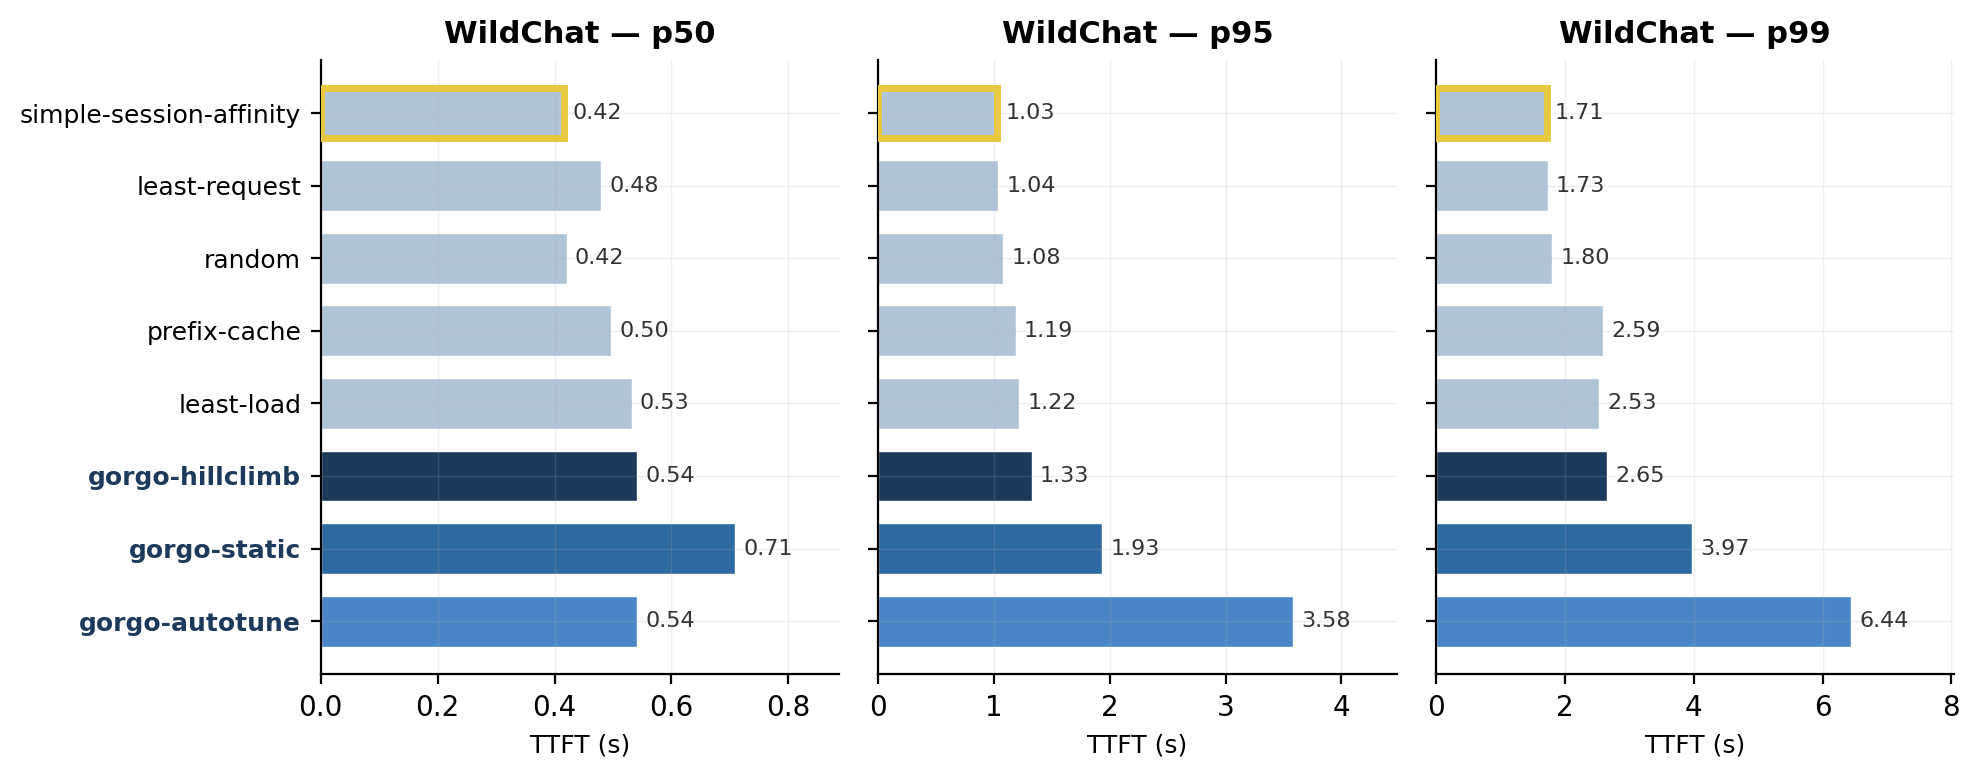
\includegraphics[width=\linewidth]{ttft_bars_wildchat.png}
\caption{WildChat-4.8M replay, per-percentile TTFT (p50/p95/p99) across
  the eight policies. GORGO variants (dark blues) are not competitive:
  \texttt{gorgo-static} and \texttt{gorgo-autotune} are the slowest two
  policies at the tail, and \texttt{gorgo-hillclimb} sits mid-pack. The
  ranking inverts the ARTChat-411k result, consistent with the regime
  argument in \S\ref{sec:characterization}.}
\label{fig:ttft_bars_wildchat}
\end{figure}

The ranking is reversed: \texttt{simple-session-affinity} wins p95 and
p99 by a large margin, \texttt{least-request} is competitive,
\texttt{gorgo-hillclimb} sits mid-pack, and \texttt{gorgo-static} and
\texttt{gorgo-autotune} are the worst two policies. Two mechanisms drive
this. First, the prefill term in Equation~\ref{eq:score} is small at
2{,}925 tokens; the cost-model weights are mostly fitting noise.
Second, intra-user reuse is 5.3\% rather than 53\%; even a perfect
cache-routing decision saves only a few hundred tokens per request, well
inside the cross-region RTT band, so chasing cache locality is
counterproductive when paired with a cross-region routing penalty. The
\texttt{gorgo-static} weights frozen from an ARTChat-411k W1 are particularly
mis-calibrated to this regime---a reminder that the cost-model parameters
do not transfer across workload classes.

We include this result as a regime-sensitivity control, not as a
contribution. The takeaway is the same one stated in \S\ref{sec:characterization}:
the gain from joint cache--network--queue routing depends on the workload
having long prompts and substantial intra-user prefix reuse. Public chat
datasets do not exercise this regime.

\section{GORGO Achieves Convergence of Cache Reuse}
\label{app:convergence}

\begin{figure}[h]
\centering
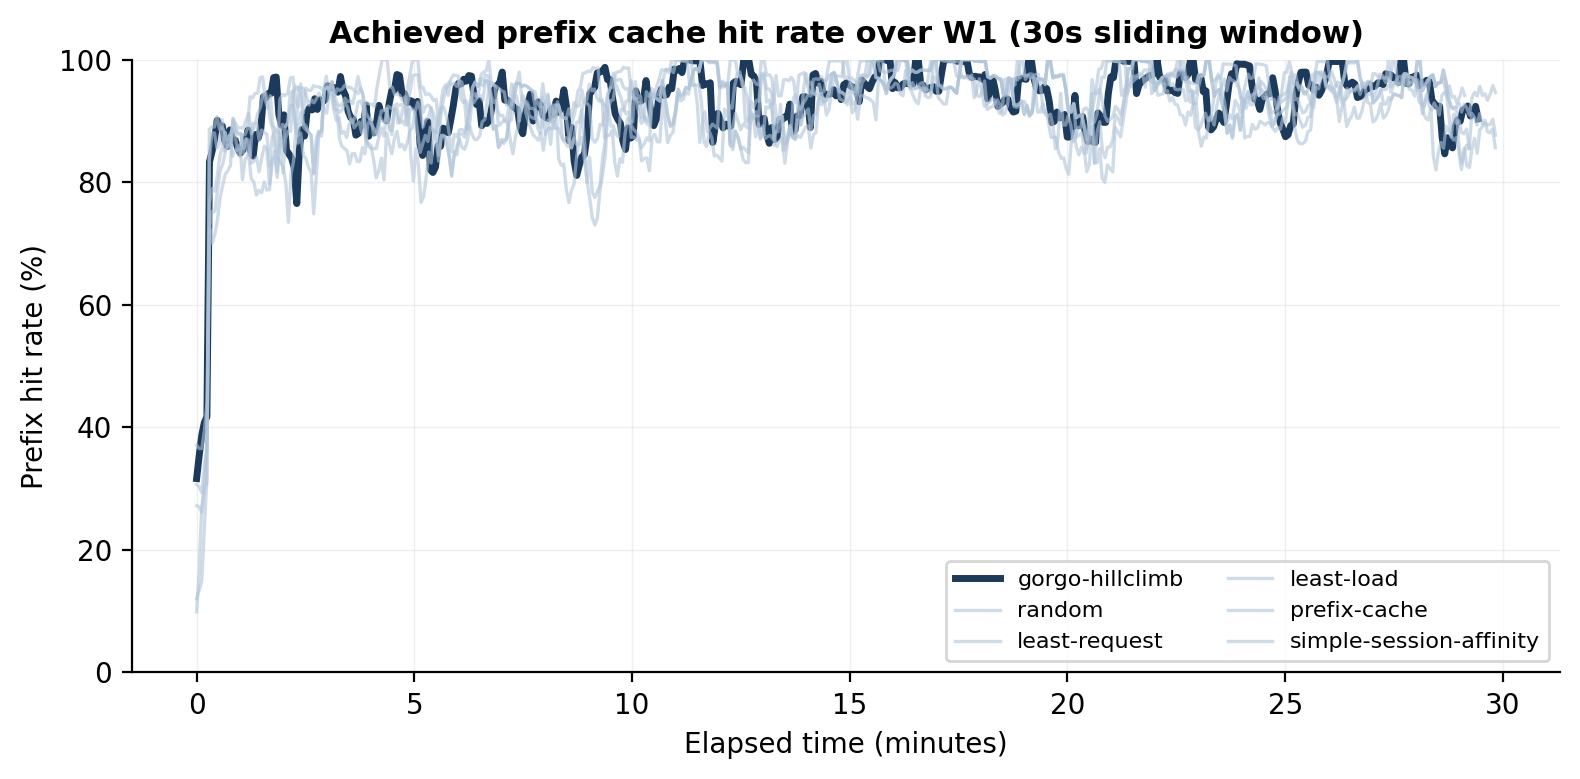
\includegraphics[width=0.75\linewidth]{cache_convergence.png}
\caption{Achieved prefix hit rate over the W1 tuning window: the fraction
  of each request's input tokens that were already cached on the replica
  the policy routed to (not the total cache available across all replicas).
  A higher rate means the routing decision exploited more of the available
  cache. Bold lines are EWMA-smoothed ($\alpha{=}0.06$); faint lines are
  64-request rolling averages. \texttt{gorgo-hillclimb} converges from
  $\sim$45\% to $\sim$95\% within the first 5 minutes as the ES learns
  to route requests to their best-cached replica.}
\label{fig:cache_convergence}
\end{figure}

\section{Load-Weight Ablation: Single-Replica Concentration}
\label{app:load_ablation}

When $w_{\mathrm{load}}$ is unconstrained (range $[10^{-5}, 5]$), the ES
drives it to zero: the resulting policy routes 100\% of traffic to a single
replica (Figure~\ref{fig:load_ablation}). On the nighttime tuning trace
($\sim$1.2\,req/s) this produces the best TTFT because every request hits
a warm cache on the closest replica with no load penalty. On the heavier
midday diurnal trace ($\sim$1.7\,req/s, 47\% more requests), the single
replica saturates: decode throughput drops to 70\,tok/s (vs.\ 119\,tok/s
with $w_{\mathrm{load}}{=}6.38$) and E2E p95 inflates to 12.58\,s---4.8$\times$
worse than \texttt{least-request}.

Constraining the ES search range to $w_{\mathrm{load}} \in [0.1, 10.0]$
prevents this degenerate solution. The ES converges to
$w_{\mathrm{load}}{\approx}6.38$, which actively avoids loaded replicas and
achieves the best TTFT \emph{and} E2E on both evaluation windows
(\S\ref{sec:results:p95}). Table~\ref{tab:load_ablation} compares the two
configurations on the midday diurnal trace.

\begin{table}[h]
\centering
\small
\caption{Midday diurnal evaluation: unconstrained ($w_{\mathrm{load}}{=}0$)
  vs.\ constrained ($w_{\mathrm{load}}{=}6.38$) \texttt{gorgo-static}.
  Constraining $w_{\mathrm{load}}$ trades 3\% TTFT p95 for 5$\times$ better
  E2E p95.}
\label{tab:load_ablation}
\begin{tabular}{lrrrrrr}
\toprule
 & TTFT p50 & TTFT p95 & E2E p50 & E2E p95 & Decode & Concentration \\
\midrule
$w_{\mathrm{load}}{=}0$    & \textbf{0.190} & \textbf{1.101} & 2.07 & 12.58 & 70  & 100\% \\
$w_{\mathrm{load}}{=}6.38$ & 0.195          & 1.136          & \textbf{1.29} & \textbf{2.46} & \textbf{119} & 60\% \\
\midrule
$\Delta$ & +2.6\% & +3.2\% & $-$37.7\% & $-$80.4\% & +70\% & \\
\bottomrule
\end{tabular}
\end{table}

\begin{figure}[h]
\centering
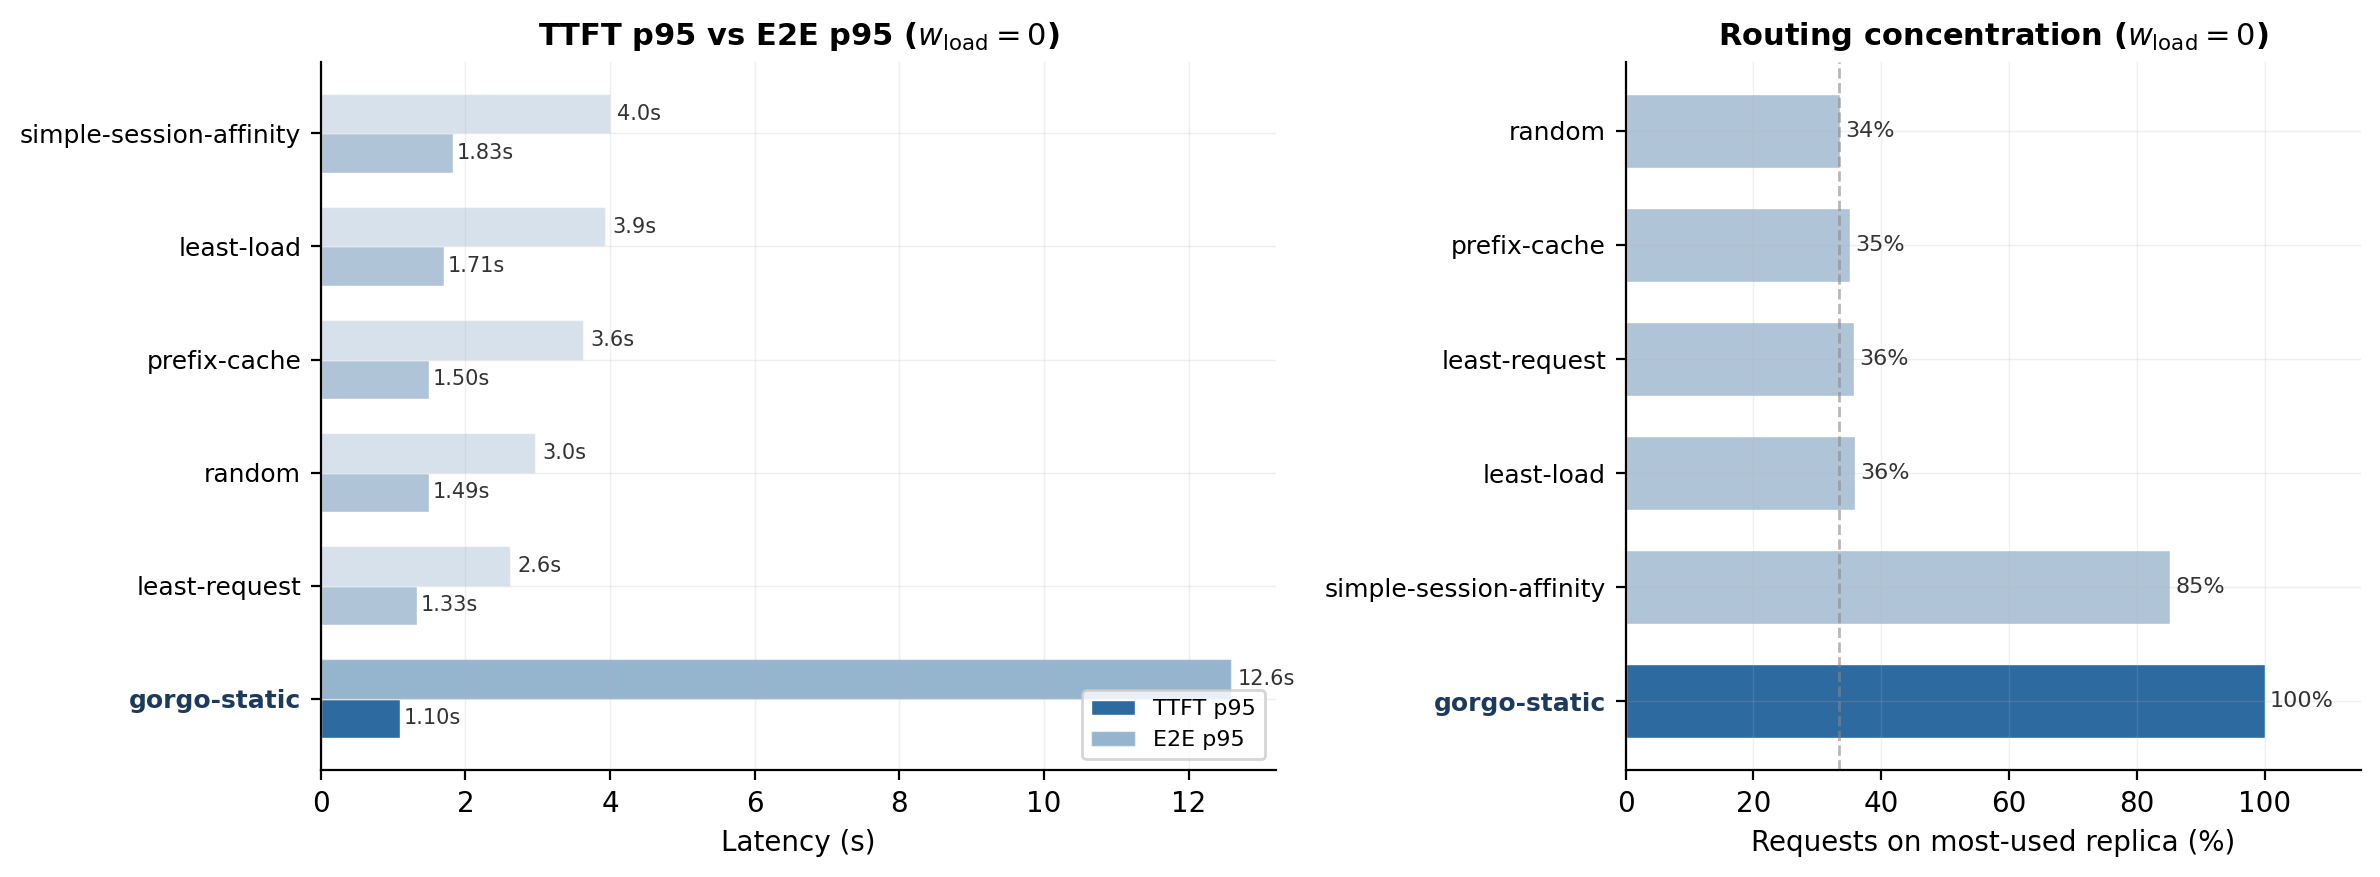
\includegraphics[width=\linewidth]{load_weight_ablation.png}
\caption{\textit{Left}: TTFT p95 (dark) vs.\ E2E p95 (light) on the midday
  diurnal trace with $w_{\mathrm{load}}{=}0$. \texttt{gorgo-static} wins
  TTFT but its E2E inflates to 12.6\,s. \textit{Right}: routing concentration.
  \texttt{gorgo-static} sends 100\% of requests to one replica.}
\label{fig:load_ablation}
\end{figure}

\end{document}